\section{Development}

\subsection{Cache}
\dots

\subsection{Motion capture}
\begin{center}
	\begin{figure}[ht!]
		\makebox[\textwidth]{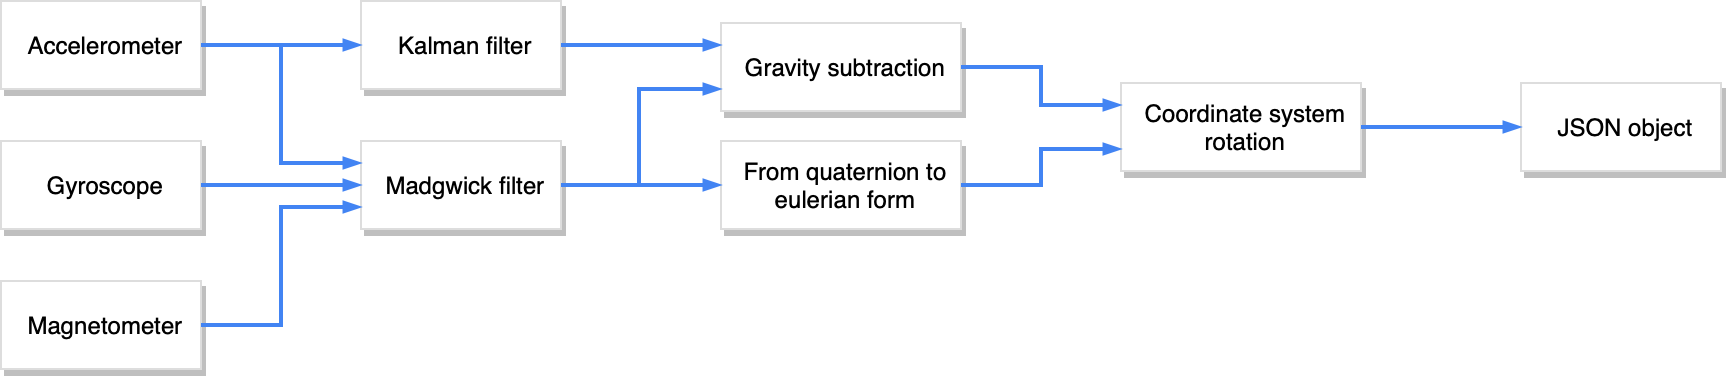
\includegraphics[width=0.50\paperwidth]{img/data_fusion.png}}
		\caption{Data fusion schema.}
	\end{figure}
\end{center}

For a better training of the neural network, the main problem was to achieve the cleanest data from the sensors. Previously, the data collected were:
\begin{itemize}
	\item yaw, pitch and roll angles;
	\item accelerations in spherical coordinates system;
	\item raw gyroscope data;
	\item a velocity approximation.
\end{itemize}
\bigbreak

Through preliminary tests has been discovered that acceleration values included gravity; thus it was necessary a more complex training data collection, due to the lack of orientation invariance (in order to obtain such invariance it would have been necessary to collect every pattern with the toy rotated in any possible angle).

Nevertheless, gravity-free acceleration data were computed by the device (with the help of the Madgwick's fusion algorithm output) and sent to the server but not stored in the database, only used for the 3D visual representation, both in training and session recording phase. It was decided to keep such data and analyze it to see if it was reliable over time.
\bigbreak

Some testing showed quickly that there was an error in the yaw angle calculation: the more the toy was rotated (regardless of the axis), the more the yaw diverged. Such error was initially imputed to the Madgwick algorithm implementation, more precisely to the convergence of its error-correction gradient descent algorithm.

Unfortunately, different algorithm implementations and different values of the algorithm's gain parameter (the magnitude $\beta$ of the gyroscope measurement error\footnote{Increasing $\beta$ leads to faster bias corrections and higher sensitiveness to lateral accelerations.} [CITE]) have no given better results over time, and worse, sometimes ghost accelerations were found.

During the tests, it was noticed that recordings of the same pattern with different device orientations didn't split the acceleration differently among axes, revealing that the reference system was integral with the Earth's center instead of the device's sensor center. To align it back, the acceleration vector has been rotated using a 3D rotation matrix. The 3 rotation angles are given by the Madgwick algorithm in the quaternion form, then converted to the eulerian one.
\bigbreak

A \textit{yaw} is a CCW rotation of $\alpha$ on the $z$-axis. The rotation matrix is
\[
	R_z(\alpha) =
	\begin{pmatrix}
		\cos\alpha & -\sin\alpha & 0 \\
		\sin\alpha & \cos\alpha & 0 \\
		0 & 0 & 1
	\end{pmatrix}
\]
Note that the upper left values compose a 2D rotation matrix, and the coordinates on the third dimension (around whom the rotation happens) are left unchanged. The same applies to the other two matrices, but with the second and the first dimension.
\bigbreak

A \textit{pitch} is a CCW rotation of $\beta$ on the $y$-axis. The rotation matrix is
\[
	R_y(\beta) =
	\begin{pmatrix}
		\cos\beta & 0 & \sin\beta \\
		0 & 1 & 0 \\
		-sin\beta & 0 & \cos\beta
	\end{pmatrix}
\]

A \textit{roll} is a CCW rotation of $\gamma$ on the $x$-axis. The rotation matrix is
\[
	R_x(\gamma) =
	\begin{pmatrix}
		1 & 0 & 0 \\
		0 & \cos\gamma & -\sin\gamma \\
		0 & sin\gamma & \cos\gamma
	\end{pmatrix}
\]
\begin{gather*}
	R(\alpha, \beta, \gamma) = R_z(\alpha) R_y(\beta) R_x(\gamma) = \\
	\begin{pmatrix}
		\cos\alpha \cos\beta & \cos\alpha \sin\beta \sin\gamma - \sin\alpha \cos\gamma & \cos\alpha \sin\beta \cos\gamma + \sin\alpha \sin\gamma \\
		\sin\alpha \cos\beta & \sin\alpha \sin\beta \sin\gamma + \cos\alpha \cos\gamma & \sin\alpha \sin\beta \cos\gamma - \cos\alpha \sin\gamma \\
		-\sin\beta & \cos\beta \sin\gamma & \cos\beta \cos\gamma
	\end{pmatrix}
\end{gather*}
It is important to note that $R(\alpha, \beta, \gamma)$ performs the roll first, then the pitch, and finally the yaw. If the order of these operations is changed, a different rotation matrix would result [CITE].
\bigbreak

Given an acceleration vector $\vec a$, the rotated one is $\vec a_r = R(\alpha, \beta, \gamma) \vec a$.
The matrix-vector multiplication doesn't need specific optimizations in the code because the dimensions at stake are too small for a meaningful speed or space improvement, and however the C++ code is compiled by \texttt{GCC} with the \texttt{-Os} flag, that includes the loop unrolling optimization [CITE].
\bigbreak

At this point, both problems were solved: the coordinate system was integral with the toy, and the yaw angle was calculated correctly.
\bigbreak

Once achieved a reliable gravity-filtered acceleration approximation, it was possible to do some fine tuning. Calibration, hard and soft iron.

The velocity approximation was excluded by the training set because\dots
\bigbreak

\subsection{Delay in real-time data plotting}
\dots
